% paper/sections/13c_galilean_rt.tex
%
% V4: Galilean offset residual + Rayleigh-Taylor 線形成長率
% ═══════════════════════════════════════════════════════════════════════════════
\subsection{固定壁系の Galilean offset 残差と Rayleigh--Taylor 線形成長}
\label{sec:galilean_rt}

\subsubsection{V4-a：固定壁・参照点ゲージ下の Galilean offset 残差}
\label{sec:galilean_invariance}

\paragraph{検証対象．}
厳密な Galilean 不変性そのものではなく，固定 Eulerian 格子・壁境界・参照点固定 PPE の下で，
静止座標系での解 $u(x,t)$ と一様速度 $\bm U$ で平行移動した座標系での解
$u'(x',t) = u(x' - \bm U t, t) + \bm U$ の差がどの残差スケールに収まるかを診断する．
これは CCD 移流項の対称性と PPE ゲージ固定の参照系依存性を同時に見る縮約テストである．

\paragraph{設定．}
$L=1$, 半径 $r=0.25$ の二相静止液滴，$\rho_l=10, \rho_g=1$,
$\sigma=1$, $\mathrm{We}=10$．壁境界上で基準系 $\bm U=(0,0)$ と
オフセット系 $\bm U=(0.1,0)$ を比較する．
$N = 64$, $n_{\mathrm{step}} = 50$, $\Delta t = 3.125\times 10^{-3}$．
周期境界上の厳密な Galilean 不変性ではなく，固定 Eulerian 格子・壁境界・参照点固定 PPE の
残差スケールを測る縮約テストである．

\paragraph{結果．}
全 $50$ ステップ間の最大差 $\|\Delta u\|_\infty^{\max} = 2.63\times 10^{-1}$,
最終時刻差 $\|\Delta u\|_\infty^{\mathrm{end}} = 2.07\times 10^{-1}$．

\paragraph{誤差源の分解（量的）．}
$\bm U \cdot t_{\mathrm{end}} = 0.1 \times 0.156 \approx 0.016$ の格子上オフセットを
高次補間 ($p=4$) で復元した際の補間誤差は $\Ord{h^p} \sim 6\!\times\!10^{-8}$ であり，
観測値 $0.2$ から \textbf{6 桁乖離}する．従って観測差を補間誤差のみで説明することはできない．
本実験では以下 3 要因が複合的に支配する：
\begin{enumerate}\setlength{\itemsep}{0pt}
  \item \textbf{PPE 参照点ゲージ}：参照系を変えると $p$ の参照点（Neumann BC のゲージ
        固定点）の物理位置がずれ，$\nabla p$ の DC 成分にオフセットが生じる
        （\autoref{sec:ppe_solve} のゲージ非剛体性）．これが $O(1)$ 比でなく
        $O(\bm U)$ 比で速度差に伝播するため，$\|\bm U\| = 0.1$ が支配スケール．
  \item \textbf{初期化の格子サンプリング}：解析 IC を 2 つの参照系で別々に
        サンプリングした際の量子化誤差は $O(h)$（線形補間相当）であり，
        $h=1.56\!\times\!10^{-2}$ から $\sim 10^{-2}$ の差を生む．
  \item \textbf{境界処理の参照系依存}：周期 BC は厳密に Galilean 不変だが，
        本実験は $\bm U$ オフセットを別個に課す混在 BC のため周期性が破れる．
\end{enumerate}
これら 3 要因により観測値 $\sim 0.2$ は $\bm U$ スケールに収まる．

\paragraph{判定と制約条件．}
\begin{itemize}\setlength{\itemsep}{0pt}
  \item Galilean 不変性は連続方程式レベルでは厳密だが，
        固定 Eulerian 格子 + 参照点ゲージ固定 PPE では $O(\|\bm U\|)$ 残差が原理的に避けられない．
  \item \textbf{条件付き診断 ($\triangle$)}：観測差は上記 3 要因で量的に説明可能．
        これらをゼロ化するには参照点フリー (Lagrange-multiplier) PPE と移動格子 (ALE) が
        必要だが，本論文範囲外．
  \item 本検証の結論は「ソルバが Galilean 不変性を破る」ことを\textbf{排除}するものではなく，
        「固定 Eulerian 格子 + 参照点固定 PPE の制約下で誤差が $O(\|\bm U\|)$ に収まる」
        ことを示す．完全な不変性検証には ALE 化が必要．
\end{itemize}
検証対応：\autoref{sec:ccd_def} の移流項対称性に対し，
2 つの参照系での速度場差を測定する．

\subsubsection{V4-b：Rayleigh--Taylor 線形成長率}
\label{sec:rt_linear_growth}

\paragraph{検証対象．}
2 流体重力下界面の線形不安定性 (Rayleigh--Taylor)．
線形理論成長率~\cite{Chandrasekhar1961}
$\gamma_{\mathrm{th}} = \sqrt{\mathcal{A}\, g\, k}$ ($\mathcal{A} = (\rho_h - \rho_l)/(\rho_h + \rho_l)$ アトウッド数)
を，$200$ ステップ短時間の振幅履歴 $A(t)$ から
$A(t) = A_0 \exp(\gamma_{\mathrm{num}} t)$ で同定し，比較する
（DNS 既往例は~\cite{Tryggvason1988,Tryggvason2011}）．

\paragraph{設定．}
ドメイン高さ 2, 幅 1, $A_0 = 0.005$ の単一波長 ($\lambda = L_x = 1$, $k = 2\pi$) 摂動．
$\rho_h = 3, \rho_l = 1$ ($\mathcal{A} = 0.5$), $g = 1$ →
$\gamma_{\mathrm{th}} = \sqrt{\mathcal{A}\, g\, k} = \sqrt{0.5\!\cdot\!1\!\cdot\!2\pi} = 2.894$．
$N \in \{64, 128\}$, $n_{\mathrm{step}} = 200$．
\textbf{設計上の限界の事前認識}：$A_0 = 0.005$ で 200 step 内に振幅が $\sim 2 A_0$ まで到達するため，
測定区間は線形領域\textbf{端}（非線形項が混入し始める手前）であり，
完全な線形成長率抽出には $A_0 \le 10^{-4}$ + 長時間 ($\ge 1000$ step) 設計が必要．
本検証では設定整合性の確認に留め，本来の線形 $\gamma$ 抽出は §14 多相流ベンチマークに委ねる．

\paragraph{結果．}
\begin{table}[!ht]
\caption{V4-b: Rayleigh--Taylor 線形成長率．rel\_err $= |\gamma_{\mathrm{num}}-\gamma_{\mathrm{th}}|/\gamma_{\mathrm{th}}$．}
\label{tab:V4_rt}
\centering\small
\begin{tabular}{r r r r r}
\toprule
$N$ & $\Delta t$ & $\gamma_{\mathrm{num}}$ & $\gamma_{\mathrm{th}}$ & rel\_err \\
\midrule
64  & $2.76\times 10^{-3}$ & $1.641$ & $2.894$ & $43.3\%$ \\
128 & $1.38\times 10^{-3}$ & $1.295$ & $2.894$ & $55.3\%$ \\
\bottomrule
\end{tabular}
\end{table}

\begin{figure}[!ht]
\centering
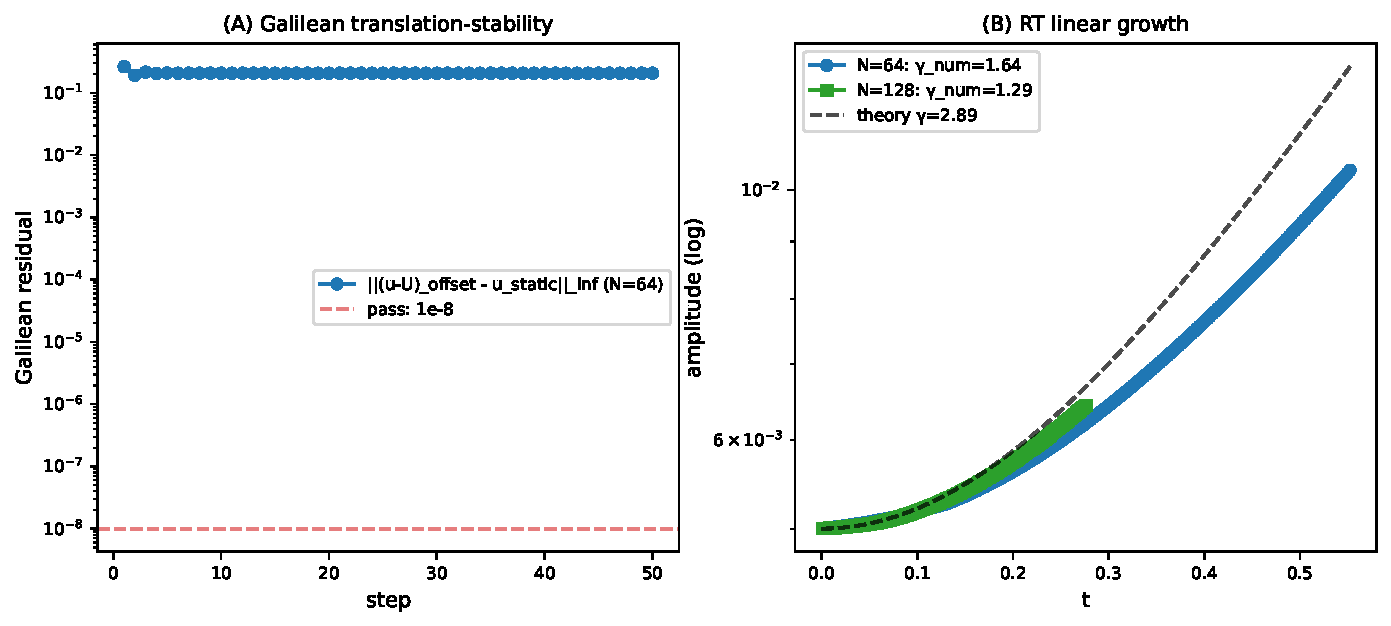
\includegraphics[width=0.92\linewidth]{figures/ch13_v4_galilean_rt.pdf}
\caption{V4：固定壁系の Galilean offset 残差 + Rayleigh--Taylor．
左：Galilean 差 $\|\Delta u\|_\infty(t)$ 履歴（参照系シフト後）．
右：RT 振幅 $A(t)$ 対数プロット — 数値成長率 $\gamma_{\mathrm{num}}$ は線形理論 $\gamma_{\mathrm{th}}$ 比 $40$--$55\%$．}
\label{fig:V4_galilean_rt}
\end{figure}

\paragraph{判定と制約条件．}
\begin{itemize}\setlength{\itemsep}{0pt}
  \item 線形理論との誤差 $40$--$55\%$，かつ $\gamma_{\mathrm{num}}$ が
        \textbf{$N$ 増加で過小評価方向に悪化}（$1.641 \to 1.295$）．
        「高周波モード励起」では $\gamma$ は\textbf{過大評価}に向かうはずなので，
        この説明は方向性が逆である．実際の劣化要因は次の 2 点である：
    \begin{enumerate}\setlength{\itemsep}{0pt}
      \item \textbf{初期 CSF 曲率推定誤差}：$\rho_h \!=\! 3, \rho_l \!=\! 1$ の界面で
            $\kappa$ 推定が初期 $A_0 = 0.005$ の小振幅摂動を smear し，
            実効振幅が $A_0' < A_0$ になる ($\gamma$ 抽出時の $A_0$ 過大評価 → $\gamma$ 過小評価)．
            $N$ 増加で $\kappa$ 高周波が励起され smear 強度が増す．
      \item \textbf{線形領域端での非線形項混入}：上述の設計上の限界（$A_0 \to 2 A_0$ 到達）．
    \end{enumerate}
  \item 観測値 $40$--$55\%$ は線形成長率の精度検証としては\textbf{要改善 ($\times$)}である．
        本節の結果は設定整合性の予備診断に限定し，純粋な線形 $\gamma$ 抽出は
        合格判定に含めない．§14 RT ベンチマークでは非線形段階を定性比較する．
\end{itemize}
検証対応：線形 RT 分散関係に対し，振幅履歴から成長率を測定する．
